\documentclass[
    paper=a4,
    % fontsize=12,
    % DIV=calc,
]{scrartcl}

\usepackage[T1]{fontenc}	
\usepackage[utf8]{inputenc}
\usepackage[ngerman]{babel}
\usepackage{microtype}
\usepackage{libertine}
\usepackage[libertine]{newtxmath} 

\usepackage{xcolor}
\usepackage{booktabs}
\usepackage{graphicx}
\usepackage{subcaption}
\usepackage{pdfpages}
\usepackage{svg}
\usepackage[
    locale		=	DE, 					%	Deutsche Normen
	detect-all,								%	Richtige Font im Textmodus/Mathemodus
	per-mode	=	fraction,				%	Bruchstrich darstellen
	range-units	=	repeat,					%	Einheiten wiederholt darstellen bei sirange
	range-phrase=	{{ bis }},	
]{siunitx}
\usepackage{amsmath}
\usepackage{circuitikz}


\usepackage{hyperref}

\definecolor{colorblue}{HTML}{0480CC}				% color for weblinks
\definecolor{colordarkblue}{HTML}{4C1DCC}			% no use case at the moment
\definecolor{colorgreen}{HTML}{26CC1B}				% color for missing macro
\definecolor{colorred}{HTML}{CC1204}				% color for edit macro


\KOMAoptions{
    numbers=noendperiod,
}

\hypersetup{
    bookmarksnumbered   =   true,
    breaklinks          =   true,
    colorlinks          =   true,
    linkcolor           =   colorred,
    urlcolor            =   colorblue,
    pdftitle            =   {Labor 3 Jan Hoegen},
    pdfsubject          =   {Versuchsvorbereitung Labor Digitaltechnik},    
    pdfauthor           =   {Jan Hoegen},
}

\ctikzset{
    logic ports=european,
    logic ports/scale=1.0,
    logic ports/fill=lightgray,
    tripoles/european not symbol=ieee circle,
}
\usetikzlibrary{babel}

\graphicspath{/Anhang}

\newcommand{\shadowsection}[1]{%
	\refstepcounter{section}
	\addcontentsline{toc}{section}{\protect\numberline{\thesection}{#1}}
}

\newcommand{\legend}[1]{\par\footnotesize\textbf{Legende}: #1\par}
\newcommand{\figsource}[1]{\par\footnotesize\textbf{Quelle:} #1\par}

\newcommand{\quoteenv}[1]{\glqq #1\grqq} 

\titlehead{
    \textsc{Hochschule Karlsruhe}\\
    University of Applied Sciences\\
    Studiengang EITB SS 22}
\subject{Digitaltechnik Labor 3}
\title{Würfel: Taktgefühl und Gedächtnis}
\subtitle{Vorbereitung}
\author{Jan Hoegen\thanks{Matrikelnumer: 82358}}
\publishers{Betreuer: Prof. Dr.\,-Ing. Jan Bauer}
\date{Erstellt am: \today}


\begin{document}

\maketitle

\tableofcontents

\newpage

\section{Binärdarstellung des Geburtstages}
    Das Ergebnis der XOR-Schaltung mit 4 Eingängen wird genau dann 1, wenn die Anzahl der high-gesetzten Eingangsvariablen ungerade ist.

    In einer Zweiergruppe mit Rithik Kumar bilden sich die Binärzahlen aus Tabelle \ref*{tab:1}.
    
    \begin{table}[h]
        \centering
        \caption{Binärdarstellung des zusammengesetzten Geburtstages}
        \label{tab:1}
        \begin{tabular}{lll}\toprule
            Name                &   Tag     &   Monat\\\midrule
            Jan Hoegen          &   22      &   11\\
            Rithik Kumar        &   02      &   01\\\midrule
            Summe               &   24      &   12\\
            Binärdarstellung    &   11000   &   1100\\\bottomrule
        \end{tabular}
    \end{table}

    Das Rechenergebnis für Monat und Tag ist:
    \begin{align*}
        P_T=& 1 \oplus 1 \oplus 0 \oplus 0 \oplus 0 = 0\\
        P_M=& 1 \oplus 1 \oplus 0 \oplus 0 = 0
    \end{align*}
        
    Damit ist der Tetraeder in FULL-NAND zu erstellen.

\section{Der Zähler}
    Der Zähler muss 5 Zustände abbilden können (die Zahlen 0 bis 4). Diese Zahlen lassen sich in 3 Bits darstellen, dementsprechend werden 3 Flip-Flops benötigt. Abbildung \ref{fig:1} zeigt das Zustandsdiagramm des Zählers. In Abbildung \ref{fig:2} wird die Struktur mit einem Übergangsschaltnetz beschrieben.
    
    \begin{figure}[h]
        \centering
        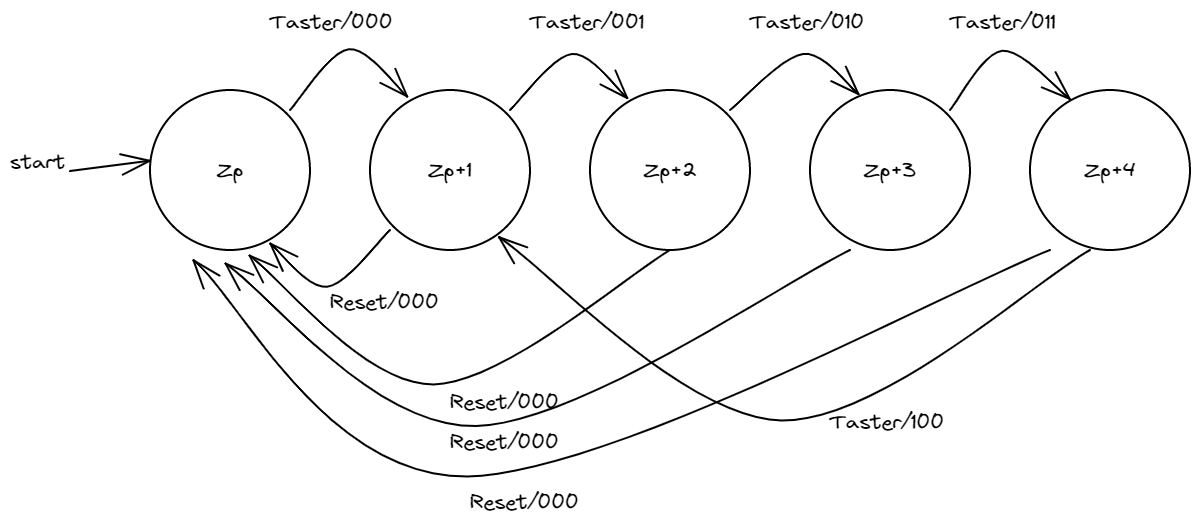
\includegraphics[width=0.8\textwidth]{Zustandsdiagramm.png}
        \caption{Zustandsdiagramm des Zählers}
        \label{fig:1}
    \end{figure}

    \begin{figure}
        \centering
        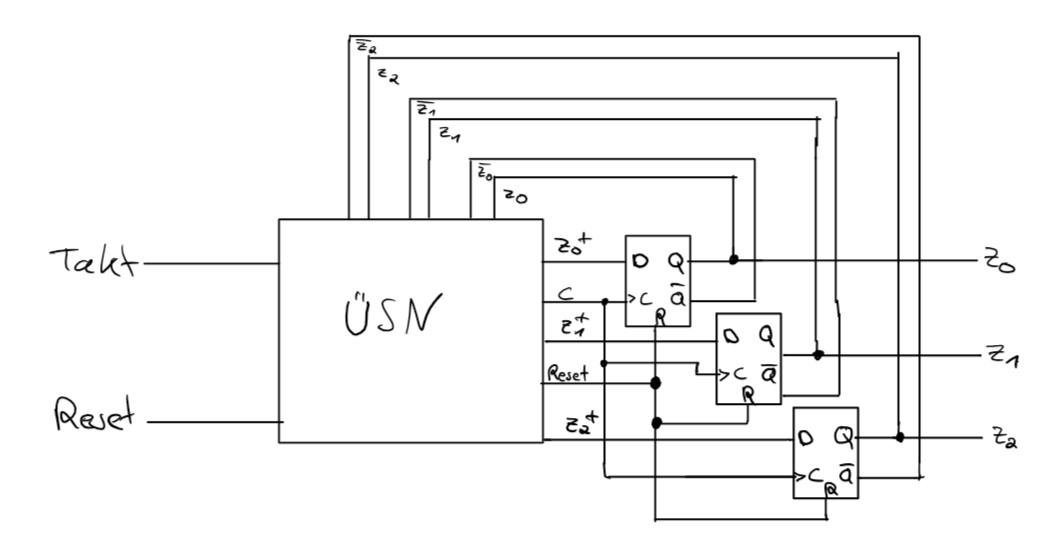
\includegraphics[width=0.8\textwidth]{Block.jpg}
        \caption{Schaltstruktur des Zählers}
        \label{fig:2}
        \legend{ÜSN: Übergangsschaltnetz}
    \end{figure}

\section{Zustandsübergangstabelle}
    Zur Darstellung der Ziffern wird die Zustandsübergangstabelle in Tabelle \ref{tab:2} aufgestellt. Es gelten die Deklarationen aus Abbildung \ref{fig:2}.

    \begin{table}[h]
        \centering
        \caption{Zustandsübergangstabelle des Zählers}
        \label{tab:2}
        \begin{tabular}{r|*{3}{l}|l|*{3}{l}|*{3}{l}}\toprule
            Zählwert    &   $Z_2$   &    $Z_1$  &    $Z_0$  &   $E$     &   $Z_2^+$ &   $Z_1^+$ &   $Z_0^+$ &   $A_2$   &   $A_1$   &   $A_0$\\\midrule
            0           &    0      &   0       &   0       &   0       &   0       &   0       &   0       &   0       &   0       &   0\\
            0           &   0       &   0       &   0       &   1       &   0       &   0       &   1       &   0       &   0       &   1\\
            1           &   0       &   0       &   1       &   0       &   0       &   0       &   1       &   0       &   0       &   1\\
            1           &   0       &   0       &   1       &   1       &   0       &   1       &   0       &   0       &   1       &   0\\
            2           &   0       &   1       &   0       &   0       &   0       &   1       &   0       &   0       &   1       &   0\\
            2           &   0       &   1       &   0       &   1       &   0       &   1       &   1       &   0       &   1       &   1\\
            3           &   0       &   1       &   1       &   0       &   0       &   1       &   1       &   0       &   1       &   1\\
            3           &   0       &   1       &   1       &   1       &   1       &   0       &   0       &   1       &   0       &   0\\
            4           &   1       &   0       &   0       &   0       &   1       &   0       &   0       &   1       &   0       &   0\\
            4           &   1       &   0       &   0       &   1       &   0       &   0       &   1       &   0       &   0       &   1\\\midrule
            5           &   1       &   0       &   1       &   0       &   X       &   X       &   X       &   X       &   X       &   X\\
            5           &   1       &   0       &   1       &   1       &   X       &   X       &   X       &   X       &   X       &   X\\
            5           &   1       &   0       &   0       &   0       &   X       &   X       &   X       &   X       &   X       &   X\\
            6           &   1       &   0       &   0       &   1       &   X       &   X       &   X       &   X       &   X       &   X\\
            6           &   1       &   1       &   1       &   0       &   X       &   X       &   X       &   X       &   X       &   X\\
            7           &   1       &   1       &   1       &   1       &   X       &   X       &   X       &   X       &   X       &   X\\\bottomrule
        \end{tabular}
    \end{table}

\section{Minimierung der Gleichungen}
    \label{sec:1}
    Nach minimieren der Gleichungen für \(A_0, A_1, A_2\) durch KV-Tabellen und disjunktive Minimalformen und anschließende Umformung in Full-NAND ergeben sich:

    \begin{align*}
        A_0 =&   (\overline{Z_0}\wedge \overline{Z_1}\wedge E) \vee (Z_0 \wedge \overline{Z_2} \wedge \overline{E}) \vee E)\\
            =& \overline{\overline{\overline{ ( \overline{\overline{\overline{\overline{Z_0} \wedge \overline{Z_1}}} \wedge E} ) \wedge ( \overline{\overline{\overline{Z_0 \wedge \overline{Z_2}}} \wedge \overline{E}} ) }} \wedge \overline{E}}\\
        A_1 =&  (Z_0 \wedge \overline{Z_1} \wedge \overline{Z_2} \wedge E) \vee (Z_1 \wedge \overline{E})\\
            =&  \overline{ \overline{ ( \overline{\overline{ Z_0 \wedge \overline{Z_1}  ) }} \wedge \overline{\overline{ ( \overline{Z_2} \wedge E}} ) } \wedge \overline{ (Z_1 \wedge \overline{E} ) } } \\
        A_2 =&  (Z_0 \wedge Z_1 \wedge \overline{Z_2} \wedge E ) \wedge ( Z_2 \wedge \overline{E} ) \\
            =&  \overline{ \overline{ ( \overline{\overline{Z_0 \wedge Z_1}} \wedge \overline{\overline{\overline{Z_2} \wedge E}} ) } \wedge \overline{ ( Z_2 \wedge \overline{E} ) }}\\
    \end{align*}

    Für $A_0$ werden 13, für $A_1$ 10 und für $A_2$ 9 NAND-Gatter benötigt.

\section{Simulation der Schaltung}
    Die Gleichungen aus Abschnitt \ref{sec:1} ergeben das Schaltbild in Bild \ref{fig:3}. Es wurden ausschließlich NAND-Gatter verwendet, um 3 D-Flip-Flops anzusteuern. Diese werden an den BCD-zu-7-Segment-Wandler aus dem vorherigen Labor angeschlossen. Als Eingangsvariablen werden der Taster, der Taktgeber c, der Reset-button und die Zustände \(Z_0^+, Z_1^+, Z_2^+\) gewählt. Die Ausgänge der Flip-Flops können in der Simulation nicht direkt mit den zugehörigen Zustandsvariablen verbunden werden. 
    
    Die Zustände \(Z_0^+, Z_1^+, Z_2^+\) wurden mit einem Inverter verknüpft. Dies widerspricht \textit{nicht} den Anforderungen aus dem Laborbericht, denn dies ist nur das Ersatzschaltbild. Tatsächlich besitzen die D-Flip-Flops einen invertierenden Ausgang, daher ist beim realen Schaltungsaufbau kein Inverter nötig.

    Trotz intensiver Fehlersuche gibt das Simulationsergebnis die Tabelle \ref{tab:3} aus, welche offensichtlich nicht der Tabelle \ref{tab:2} entspricht. Beim ausprobieren habe ich herausgefunden, dass der Fehler vermutlich beim Taktgeber c liegt. Denn die Schaltung zeigt manuell richtige Ergebnisse an, wie der Screenshot in Abbildung \ref{fig:4} zeigt. 

    Bei weiterem ausprobieren wurde jedoch klar, dass diese Vorgehensweise nicht immer zu richtigen Ergebnissen führt. Beispielsweise führt der Eingangszustand \texttt{0011} zur angezeigten Ziffer 3. Richtig wäre an dieser Stelle die Ziffer 2. Leider war es mir trotz großer Mühe nicht möglich, den Fehler zu entdecken. Am wahrscheinlichsten ist es, dass eine falsche Verdrahtung vorliegt, ich diese aber nicht erkennen konnte.
    
    \begin{figure}[h]
        \centering
        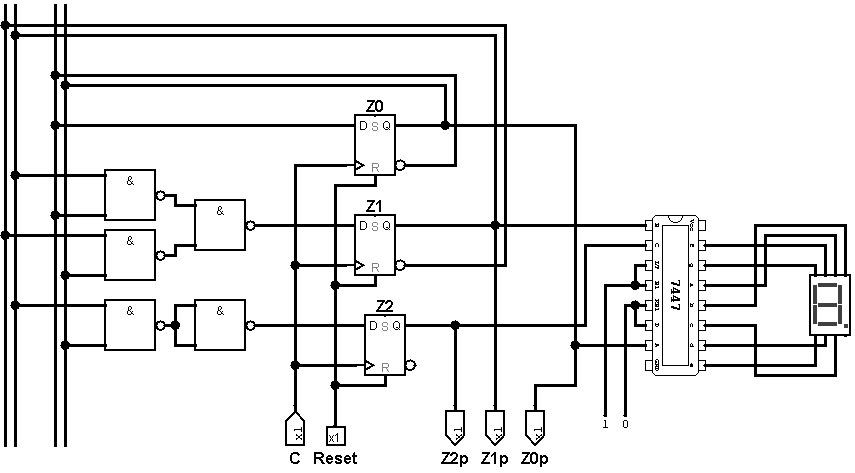
\includegraphics[width=\textwidth]{simulation.png}
        \caption{Schaltbild in Ful-NAND}
        \label{fig:3}
    \end{figure}

    \begin{table}
        \centering
        \caption{Wahrheitstabelle der simulierten Schaltung}
        \label{tab:3}
        \begin{tabular}{cccc|ccc}
            $Z2p$&$Z1p$&$Z0p$&$Taster$&$A2$&$A1$&$A0$\\
            \hline
            $0$&$0$&$0$&$0$&$0$&$0$&$0$\\
            $0$&$0$&$0$&$1$&$0$&$0$&$0$\\
            $0$&$0$&$1$&$0$&$0$&$0$&$0$\\
            $0$&$0$&$1$&$1$&$0$&$0$&$0$\\
            $0$&$1$&$0$&$0$&$0$&$0$&$0$\\
            $0$&$1$&$0$&$1$&$0$&$0$&$0$\\
            $0$&$1$&$1$&$0$&$0$&$0$&$0$\\
            $0$&$1$&$1$&$1$&$0$&$0$&$0$\\
            $1$&$0$&$0$&$0$&$0$&$0$&$0$\\
            $1$&$0$&$0$&$1$&$0$&$0$&$0$\\
            $1$&$0$&$1$&$0$&$0$&$0$&$0$\\
            $1$&$0$&$1$&$1$&$0$&$0$&$0$\\
            $1$&$1$&$0$&$0$&$0$&$0$&$0$\\
            $1$&$1$&$0$&$1$&$0$&$0$&$0$\\
            $1$&$1$&$1$&$0$&$0$&$0$&$0$\\
            $1$&$1$&$1$&$1$&$0$&$0$&$0$\\
            \end{tabular}
    \end{table}

    \begin{figure}
        \centering
        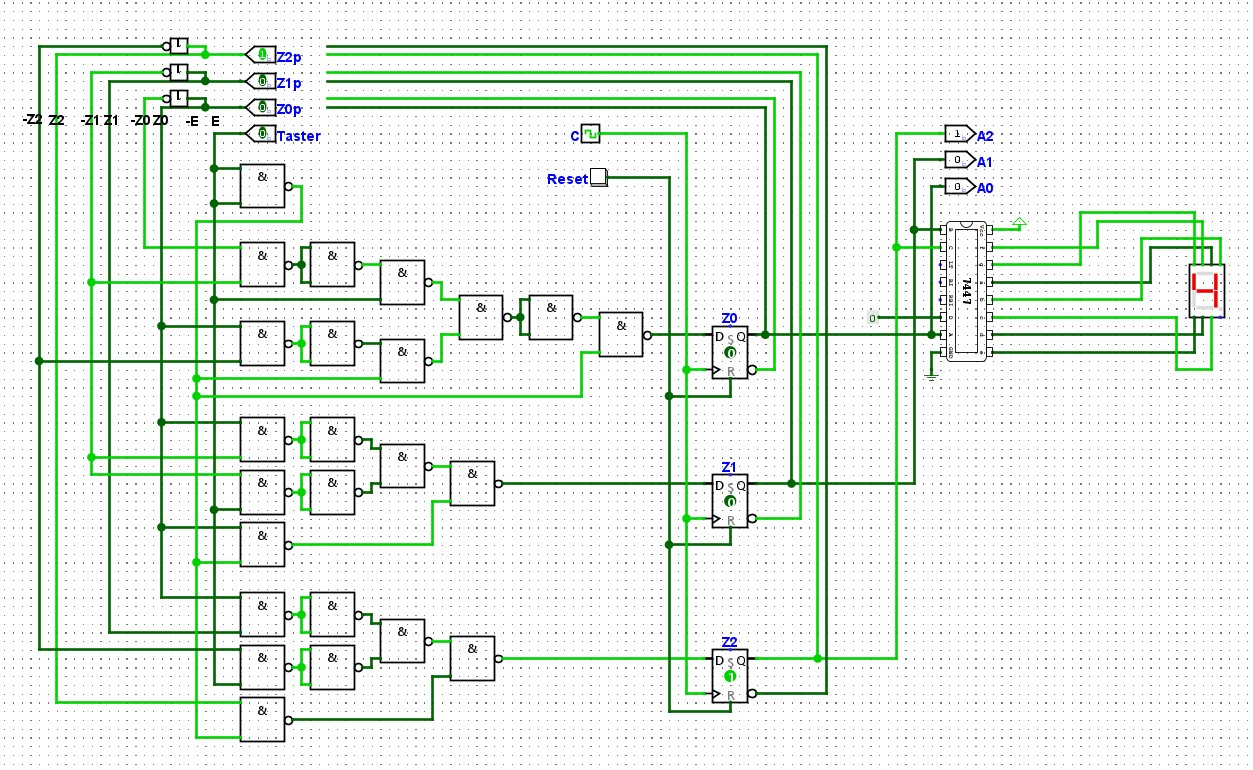
\includegraphics[width=\textwidth]{Screenshot.jpg}
        \caption{Screenshot der Simulation mit logisim-evolution}
        \label{fig:4}
    \end{figure}

\end{document}